\chapter{Results and Discussion}
\label{results_discussion}
\section{Main Results}
  % \subsection{Development Synopsis}
  %   The overall architecture of the sytem has remained largely unchanged throughout the development process. With the main exception being the decision to drop the relational database in favour of using only heirachical storage such as the filesystem and JSON files. This occured when it was established that only simple relations occured between the data and therefore adding an entire new set of dependencies and technology would be overly complex.
  \subsection{CNN}
    The Performance of the CNN given the available hardware (Google Colab GPU Runtime) is good. With a 98.6\% classification accuracy on a held out validation set. With current cutting edge being 99.74\% on the same dataset (as covered in the literature review). The CNN is capable of identifying 38 unique classes of crop images. Unfortunately due to the lack of data, one was unable to include additional defects such as lack of water/nitrogen/sunlight etc. However the design of the system allows for the CNN model to be changed very easily. As simply as changing two files on the API server. This means that as model performance improves and classification range broadens, the system is able accomodate for this.
    \par
    Seperation of the sofware components allows for the easy interchange of CNN models. This means once the model is trained, changing the model is as simple as changing a single filepath on the API server. Although if one wishes to extend the number of defects (classes) the model is able to predict; three steps must take place. Firstly, the filepath to the JSON file defining all classes must be updated on the API to reflect the new set of classes, the model .h5 file needs updating. And lastly the images for the new defect must be added to the image server. Making the process straightforward as updating two file paths and uploading images using secure file transfer protocol (SFTP).


  \subsection{Architecture}
    The seperation of responsibility between the API and front-end has created two orthogonal systems that can be upgraded and interchanged easily. The front end need not know any details about the CNN(model) it is interacting with. The classes the model is able to identify are dynamically updated on the front-end and prediction data also remains consistent between model implementations. Recourse and prevention information are similarly easy to update and can be changed dynamically, simply by updating a JSON file on the back-end. Images the front-end display are also easily changed and are hosted on a seperate image server, further seperating the systems interdependence. A call for modularity and seperation of responsibility was a key theme occuring in many works citepd in the literature review.

  \subsection{Development}
    A major change made to the design of the application was the choice to drop the relational database in favor of using heirachical storage as it was noted that the application did not need to handle complex relational data. Initially the purpose was to have the database handle filepaths to images and recourse/defect information but this was easily handled with consistent directory naming on the image server and JSON files.
    \par
    A feature that has the code in place to deliver but no infomration to display is the recourse and prevention section. At this stage one was unable to obtain the information nececarry to populate these values. However, once the relevant information is obtained, only JSON files on the API side need be updated to properly fulfill this requirement.
    \par
    Some of the main issues that arose during development were during the move to production. This involved learning new technologies such as NginX and Gunicorn to deploy the project as the configuration can be obtuse upon first interaction. Some API code also did not work the same way as on the development server and so had to be modified to work in the production environment.
    \par
    Through the use of version control it has been straightforward to update the code on the production servers as it is simple as pulling the latest changes from the git repository. version control has been helpful throught the lifecycle thanks to the ability to branch the codebase (see version control).
    \par
    Upon reflection, using the Vue.js framework standalone may not have been the best choice for the sole reason that one did not find a way of caching page states. Which has led to the inability to go back to the results display state of the Upload_Image page after navigating away from it. It is possible that using the additional Vuex library would have made this possible. Because the Upload_Image component is currently implemented with the results display state being arrived at by a series of function calls, there doesn't seem to be a vanilla Vue.js way to cache the page state to allow it to be navigated back to without starting at the initial state of the component.
    \subsection{Evaluation Results}
      \subsubsection{System Usability}
      Strongly agree = 5, Strongly disagree = 1. In the case of odd questions, agreeing is positive sentiment. For even questions agreeing is negative sentiment. The calculations are as follows. X is the sum of odd-numbered questions -5. Y is 25-sum of all even-numbered questions. The SUS score is $ (X+Y)*2.5 $ The mean average of all SUS scores is then calculated. With the best possible score being 100.
      \begin{figure}[H]
        \begin{center}
          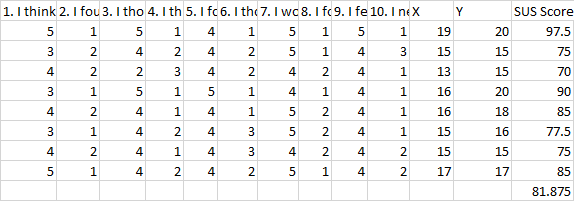
\includegraphics[scale=0.7]{Images/susScoresTable}
          \caption{SUS scores table}
          \label{fig:sus_scores_table}
        \end{center}
      \end{figure}
      In this case the system scored 81.875 which is above the average of 68 \citep{Sauro2011}. However with the limited number of questionaire respondents (8) the evidence is not wholly conclusive.
  \subsection{Requirements Checklist}
    \begin{itemize}
      \item Must Have
      \begin{itemize}
        \item CNN that is capable of classifying at least 2 different defects across 2 different plant species.\checkmark
        \item An API that allows communication from the UI to the CNN \checkmark
        \item API must be able to receive images. \checkmark
          \begin{itemize}
            \item Accepted formats being .jpg \& .png
          \end{itemize}
        \item API must return defect information, which will be an array of probability values for each defect class \checkmark
        \item API must return recourse information. \checkmark
        \item Application must display images that show the predicted defect. \checkmark
          \begin{itemize}
            \item These images may be stored either on a seperate server to the front-end. Perhaps in the API servers 'static folder'. Alternatively they will be bundled with the front end.
          \end{itemize}
      	\item The API will be robust enough to handle the receipt of erroneous requests. \checkmark
      	\item A python backend that will handle image classification using a CNN. \checkmark
      	\item A UI that will allow the user to upload an image to be analysed. \checkmark
        \begin{itemize}
          \item The user will be able to choose an image file from their local storage using a file explorer popup.
        \end{itemize}
      	\item The UI will display information regarding the likelihood of each kind of possible defect. \checkmark
      	\item To display the relevant images that fit the description of the most likely defects.\checkmark
      	\item To display recourse information to rectify the defect.\checkmark
      	\item Collecting, cleaning and pre-processing the image data. \checkmark
        \item Artificially grow the dataset by performing translations/rotations/adding noise to the images to make the training data more comprehensive.\checkmark
      \end{itemize}
      \item Should Have
      \begin{itemize}
        \item A page to allow users to see a gallery of images sorted by
          defect type. \checkmark
        \item The CNN should be able to classify at least 7 different defects across at least two different plant species. \checkmark
        \item The CNN should acheive at least 80\% accuracy at classifying all different classes of defect in a held out test set that contains an equal number of each class. \checkmark
      	\item Regularisation techniques to prvent the NN overfitting. \checkmark
      \end{itemize}
      \item Could Have
        \begin{itemize}
          \item Mobile device support. \checkmark
        \end{itemize}
      \begin{itemize}
        \item Ability for users to add additional information about the crop
          to determine the defect.
      \end{itemize}
      \item Won't Have
    \end{itemize}
